\documentclass[tikz]{standalone}

\begin{document}
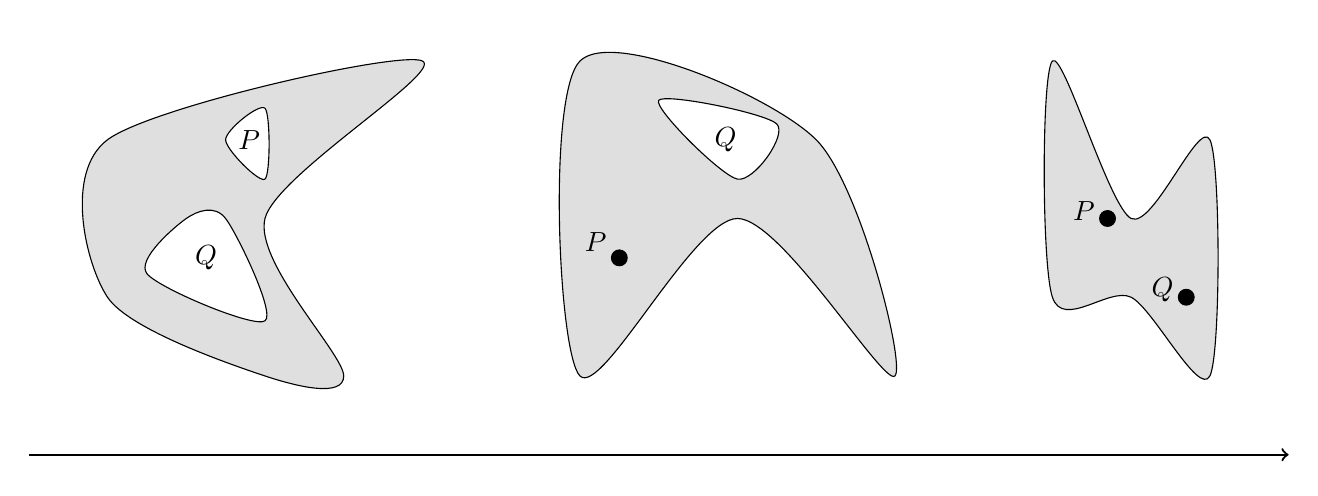
\begin{tikzpicture}

% Leftmost set and holes
\filldraw[color=lightgray!50,draw=black] plot [smooth cycle] coordinates {(-6,-2) (-5,-2) (-6,0) (-4,2) (-8,1) (-8,-1)};
\filldraw[color=white,draw=black] plot [smooth cycle] coordinates {(-6,.5) (-6,1.4) (-6.5,1)};
\filldraw[color=white,draw=black] plot [smooth cycle] coordinates {(-7.5,-.7) (-6,-1.3) (-6.5,0) (-7,0)};
\node at (-6.2,1) {\(P\)};
\node at (-6.75,-.5) {\(Q\)};

% Set with one hole contracted
\filldraw[color=lightgray!50,draw=black] plot [smooth cycle] coordinates {(-2,-2) (0,0) (2,-2) (1,1) (-2,2)};
\filldraw[color=black] (-1.5,-.5) circle (.1);
\filldraw[color=white,draw=black] plot [smooth cycle] coordinates {(0,.5) (.5,1.2) (-1,1.5)};
\node at (-1.8,-.3) {\(P\)};
\node at (-.15,1) {\(Q\)};

% Set with both holes contracted
\filldraw[color=lightgray!50,draw=black] plot [smooth cycle] coordinates {(4,-1) (5,-1) (6,-2) (6,1) (5,0) (4,2)};
\filldraw[color=black] (4.7,0) circle (.1);
\filldraw[color=black] (5.7,-1) circle (.1);
\node at (4.4,.1) {\(P\)};
\node at (5.4,-.9) {\(Q\)};

% The arrow
\draw[color=black,thick,->] (-9,-3) -- (7,-3);
% Required for the arrow to not be cut off
\node at (0,-3.05) {};

\end{tikzpicture}
\end{document}
